    
\chapter{略字 \& 幽霊字}

\begin{center}
\begin{Large}
第365課: 略字 \& 幽霊字 
\end{Large}
\end{center}
 
\par{ 略字 are unofficial variants of 漢字. 幽霊字 are characters that were supposedly accidentally created in the JIS character sets.  }
      
\section{略字}
 
\par{ There are typically two meanings of 略字. }

\begin{enumerate}

\item A generally used character shortened in handwriting. \hfill\break

\item Characters not included in the 常用漢字 list but are simplified with patterns used during script reform. \hfill\break

\end{enumerate}

\par{A very similar term is 俗字. They have circulated quite well but are not deemed proper. These characters may be called 異体字 in 漢字 dictionaries. }

\par{\textbf{EXAMPLES OF 略字 }}

\begin{ltabulary}{|P|P|P|}
\hline 

州 & 卅 & The 3 ` are changed to 一. \hfill\break
\\ \cline{1-3}

属 & 尸+虫 & The 禹 is replaced with 虫. \hfill\break
\\ \cline{1-3}

個 &  

\includegraphics[scale=0.2]{figs/第08章/第365課:_ryakujiyuureiji_fig/TRON_2_2635.png}
& 固 is replaced with 口. \\ \cline{1-3}

薄 &  & 専 is replaced with 云. Similar characters are changed likewise. \hfill\break
\\ \cline{1-3}

喜 & 七X3 & Replaced with three 七. \hfill\break
\\ \cline{1-3}

品 &  

\includegraphics[scale=0.2]{figs/第08章/第365課:_ryakujiyuureiji_fig/TRON_2_4E58.png}
& Characters with 品 are abbreviated likewise. \hfill\break
\\ \cline{1-3}

機 & 木+キ & The character may also be abbreviated with the top right part changed to 

\includegraphics[scale=0.2]{figs/第08章/第365課:_ryakujiyuureiji_fig/TRON_3_EC6C.png}
. \\ \cline{1-3}

劇 & 虎+リ & 豕 is taken out. \\ \cline{1-3}

門 &  

\includegraphics[scale=0.2]{figs/第08章/第365課:_ryakujiyuureiji_fig/RYAKUJI_2_0000.png}
& This radical change may be applied to other characters. \hfill\break
\\ \cline{1-3}

藤 & 艸冠+ト & The grass radical + the Katakana ト. \\ \cline{1-3}

潟 & 氵+写 & Taken from the simplification of 写. \\ \cline{1-3}

層 & 尸+ソ & 曽 is replaced with the Katakana ソ. \\ \cline{1-3}

魔 & 广+マ & Also the simplification of 摩. \\ \cline{1-3}

点 & 奌 & 灬 is replaced with 大. Also happens to 魚. \\ \cline{1-3}

闘 &  

\includegraphics[scale=0.2]{figs/第08章/第365課:_ryakujiyuureiji_fig/RYAKUJI_2_0000.png}
+ 斗 & Two simplifications at once. \hfill\break
\\ \cline{1-3}

第 &  
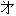
\includegraphics[scale=0.2]{figs/第08章/第365課:_ryakujiyuureiji_fig/TRON_2_243D.png}
& A simplification originating from cursive script. \\ \cline{1-3}

都 &  & 者 is changed to 土+日. \hfill\break
\\ \cline{1-3}

寸 &  & The ` is moved to the top right corner. \hfill\break
\\ \cline{1-3}

議 & 言+ギ & 義 replaced with the Katakana ギ. \hfill\break
\\ \cline{1-3}

魚 & 鱼 & 灬 replaced with 一. This can happen with any character. \\ \cline{1-3}

選 &  & 己己 replaced with ツ. \hfill\break
\\ \cline{1-3}

堅 &  & 臣 is often replaced with リ. \hfill\break
\\ \cline{1-3}

権 &  权 & Following the simplification made in China. \\ \cline{1-3}

曜 & 旺 & Pattern is not normally continued in similar characters. \\ \cline{1-3}

職 & 耺・耳+ム & Patterns are not normally continued in similar characters. \\ \cline{1-3}

衛 &  & The right half can be replace with the Katakana ヱ. \hfill\break
\\ \cline{1-3}

止 & と & This radical may be replaced with the Hiragana と. \\ \cline{1-3}

経 & 圣 & Also a common practice in replacing 軽. \\ \cline{1-3}

神 &  & 申 replaced with ヤ with ` in the lower right. \hfill\break
\\ \cline{1-3}

風 &  & Inner radical may be replaced with two `. \\ \cline{1-3}

\end{ltabulary}
\hfill\break
\textbf{Resource Note }: There are many more 略字 in existence exclusively used in Japan. However, there will be extreme personal differences, and the mentioning of them here should not be treated as a green light to use them whenever. They should only be used in personal handwriting. For those who wish to see more, visit the following page: http:\slash \slash hac.cside.com\slash bunsho\slash 1shou\slash 39setu.html       
\section{幽霊字}
 
\par{ 幽霊字 are characters found in JIS with uncertain origin, meaning, readings, or any number of these issues. The number of 幽霊字 is uncertain, and because JIS has been expanded since the initial discovery, more are bound to be discovered. It has also turned out that many 幽霊字 are actually 略字. This could give a slight reason to why they may have been added. Below is a chart with characters deemed to be 幽霊字. }

\begin{ltabulary}{|P|P|P|P|}
\hline 

垉 & ホウ & Break; collapse \hfill\break
&  \\ \cline{1-4}

壥 & テン & Shop &  \\ \cline{1-4}

彁 & カ、セイ & No meaning &  \\ \cline{1-4}

暃 & ヒ & Be separated &  \\ \cline{1-4}

汢 & ねた & Marsh &  \\ \cline{1-4}

穃 & ヨウ & No meaning &  \\ \cline{1-4}

粫 & ジ、メン、うるち & Gluten-free grain &  \\ \cline{1-4}

蟐 & ジョウ、もみ & Mantis &  \\ \cline{1-4}

鍄 & キョウ、リョウ & Clamp &  \\ \cline{1-4}

駲 & シュン、ジュン & Horse's butt &  \\ \cline{1-4}

垈 & タイ、ダイ、ぬた & Wetlands & 国字 \\ \cline{1-4}

妛 & シ、あなど(る)、おろか、みだる、みにく(い) & Ugly; contempt \hfill\break
& From a 外字 without 一 \hfill\break
\\ \cline{1-4}

恷 & キュウ、ク & Be contrary; nice &  \\ \cline{1-4}

椦 & ケン、まげもの & Wickerwork & A mistake of 橳 \\ \cline{1-4}

熕 & おおづつ & Cannon & 国字 \\ \cline{1-4}

粐 & コ、ロ、ぬか & Rice-bran &  \\ \cline{1-4}

糘 & すくも & Chaff & 国字 \\ \cline{1-4}

袮 & チ、デイ、ネ & Ancestral Shrine &  \\ \cline{1-4}

閠 & ギョク、ケイ、ジュン、うるう & Intercalation & A mistake of 閏 \hfill\break
\\ \cline{1-4}

鵈 & とび & Kite (bird) &  \\ \cline{1-4}

墸 & チョ & Hesitate & A mistake of 躇 \\ \cline{1-4}

岾 & はけ、やま & Mountain &  \\ \cline{1-4}

挧 & ウ、とち & Japanese horse chestnut &  \\ \cline{1-4}

橸 & まさ & Straight grain &  \\ \cline{1-4}

碵 & いしずえ & Cornerstone &  \\ \cline{1-4}

粭 & すくも & Chaff & 国字 \\ \cline{1-4}

膤 & セツ、そり、ゆき、たら & Snow & 国字 \hfill\break
\\ \cline{1-4}

軅 & たか、やがて & After all & A mistake of 軈 \hfill\break
\\ \cline{1-4}

靹 & ケツ、とも & Archer's arm protector & A mistake of 鞆 \\ \cline{1-4}

\end{ltabulary}
     